% Copyright (c) 2026 Mika Nystrom.  All rights reserved.

\documentclass[11pt]{article}

% Page layout
\usepackage[letterpaper, margin=1in]{geometry}
\setlength{\headheight}{14pt}
\usepackage{parskip}
\setlength{\parindent}{0pt}

% Typography
\usepackage{fancyvrb}
\usepackage{booktabs}
\usepackage{amsmath}
\usepackage{amssymb}

% Code listings
\usepackage{listings}
\lstset{
    basicstyle=\ttfamily\small,
    columns=fullflexible,
    keepspaces=true,
    showstringspaces=false,
    breaklines=true,
    frame=none,
    xleftmargin=2em,
}

% Hyperlinks
\usepackage[colorlinks=true, linkcolor=blue, urlcolor=blue, citecolor=blue]{hyperref}

% Headers and footers
\usepackage{fancyhdr}
\pagestyle{fancy}
\fancyhf{}
\fancyhead[L]{\textit{LTS Extraction from Compiled CSP Processes}}
\fancyhead[R]{\thepage}
\renewcommand{\headrulewidth}{0.4pt}

% State-transition diagrams
\usepackage{tikz}
\usetikzlibrary{automata, positioning, arrows.meta}

\title{\textbf{LTS Extraction from Compiled CSP Processes} \\[0.5em]
\large A Worked Example}
\author{Mika Nystr\"om \and Claude (Anthropic)}
\date{DRAFT Version 0.1\\
\today}

\begin{document}

\maketitle

\tableofcontents
\newpage

%======================================================================
\section{Introduction}
%======================================================================

A \emph{Labelled Transition System} (LTS) is a directed graph whose
edges are labelled with actions.  Formally, an LTS is a tuple
$(S, s_0, A, {\to})$ where $S$ is a set of states, $s_0 \in S$ is the
initial state, $A$ is an alphabet of actions, and
${\to} \subseteq S \times A \times S$ is a transition relation.
An LTS captures the externally observable behavior of a
process---which communications it can perform and in what order---while
abstracting away internal computation.

The Fulcrum CSP toolchain compiles hardware-oriented CSP descriptions
into native simulator binaries.  Simulation exercises one execution
path per run.  Formal verification requires exploration of
\emph{all} reachable states.  The first step toward this goal is
extracting an explicit LTS from each compiled process.

This document walks through a worked example: a
producer-consumer system with two processes and one channel.  We show
the CSP source, the compiled intermediate representation, the
extracted LTSs, and the Aldebaran \texttt{.aut} output format.  This
corresponds to Phase~1 of the verification roadmap described in the
\emph{Formal Verification Feasibility Study}~\cite{feasibility}.

%======================================================================
\section{The Producer-Consumer System}
%======================================================================

Our example system has two processes connected by a single channel:

\begin{itemize}
\item A \textbf{Producer} that sends incrementing integers on its
  output port~\texttt{R}.
\item A \textbf{Consumer} that receives integers on its input
  port~\texttt{L} and prints them.
\end{itemize}

%----------------------------------------------------------------------
\subsection{Process Definitions}
%----------------------------------------------------------------------

The producer (\texttt{producer.csp}):

\begin{lstlisting}
int x; *[ R!x ; x = x + 1 ]
\end{lstlisting}

This declares a local integer variable~\texttt{x} (initially zero),
then enters an infinite loop (\texttt{*[\,]}) that sends the current
value of~\texttt{x} on port~\texttt{R} and increments it.

The consumer (\texttt{consumer.csp}):

\begin{lstlisting}
int x; *[ L?x ; print(x) ]
\end{lstlisting}

This receives a value from port~\texttt{L} into local
variable~\texttt{x}, prints it, and repeats.

%----------------------------------------------------------------------
\subsection{System Description}
%----------------------------------------------------------------------

The system file (\texttt{build\_prodcons.sys}) declares the channel
and binds the ports:

\begin{lstlisting}
system ProdCons;
  var c : channel(32);

  process Producer = "producer.csp"
    port out R : channel(32);

  process Consumer = "consumer.csp"
    port in L : channel(32);

begin
  var p : Producer(R => c);
  var q : Consumer(L => c);
end.
\end{lstlisting}

The system declares a 32-bit channel~\texttt{c}, then instantiates
one Producer (binding its output port~\texttt{R} to~\texttt{c}) and
one Consumer (binding its input port~\texttt{L} to~\texttt{c}).

%----------------------------------------------------------------------
\subsection{Block Diagram}
%----------------------------------------------------------------------

\begin{center}
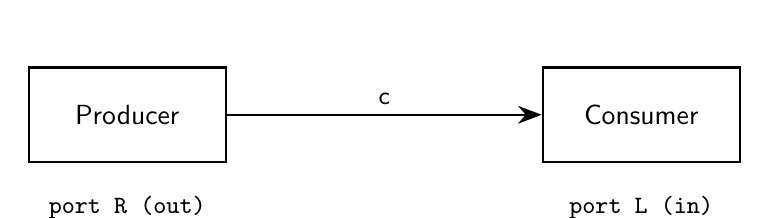
\begin{tikzpicture}[
    node distance=4cm,
    process/.style={rectangle, draw, thick, minimum width=2.5cm, minimum height=1.2cm, font=\sffamily},
    chan/.style={-{Stealth[length=3mm]}, thick},
]
  \node[process] (prod) {Producer};
  \node[process, right=of prod] (cons) {Consumer};
  \draw[chan] (prod) -- node[above, font=\sffamily\small] {c} (cons);
  \node[below=0.3cm of prod, font=\small\ttfamily] {port R (out)};
  \node[below=0.3cm of cons, font=\small\ttfamily] {port L (in)};
\end{tikzpicture}
\end{center}

The producer's output port~\texttt{R} and the consumer's input
port~\texttt{L} are both bound to channel~\texttt{c}.  When the
producer executes \texttt{R!x}, it synchronizes with the consumer's
\texttt{L?x}: data flows from producer to consumer through a
zero-slack handshake.

%======================================================================
\section{From CSP to Compiled Blocks}
\label{sec:compilation}
%======================================================================

The CSP compiler (\texttt{cspc}) transforms source code through a
multi-stage pipeline:

\begin{Verbatim}[samepage=true]
  .csp source
       |
       v
    cspfe (parser) --> S-expression AST (.scm file)
       |
       v
    cspc 9-pass compiler
       |
       v
    text9: compiled block list
\end{Verbatim}

The final output of the compiler is \emph{text9}, a list of blocks in
a normalized form.  Each block has a label (a state name), a body of
statements, and one or more \texttt{goto} targets indicating where
control transfers next.  The first element of text9 is always
\texttt{(goto START)}, naming the initial state.

%----------------------------------------------------------------------
\subsection{Producer: Compiled Blocks}
%----------------------------------------------------------------------

After compilation, the producer's text9 contains:

\begin{Verbatim}[samepage=true,xleftmargin=2em]
(goto START)

(sequence (label START)
  (var1 (decl1 (id x) (integer #f #f () ()) none))
  (assign (id x) 0)
  (goto L6))

(sequence (label L6)
  (send (id R) (id x))
  (assign (id x) (+ (id x) 10_1))
  (goto L6))
\end{Verbatim}

Reading this block by block:

\begin{description}
\item[\texttt{(goto START)}] --- The entry point.  Control begins at
  the block labelled \texttt{START}.

\item[\texttt{START}] --- Declares local variable~\texttt{x},
  initializes it to~0, then transfers to block~\texttt{L6}.
  There are no channel operations here, so the transition from
  \texttt{START} is an internal action~($\tau$).

\item[\texttt{L6}] --- Sends the value of~\texttt{x} on
  port~\texttt{R}, increments~\texttt{x}, and loops back to
  \texttt{L6}.  The \texttt{send} is the blocking operation that
  becomes the action label for this transition.
\end{description}

%----------------------------------------------------------------------
\subsection{Consumer: Compiled Blocks}
%----------------------------------------------------------------------

The consumer's text9:

\begin{Verbatim}[samepage=true,xleftmargin=2em]
(goto START)

(sequence (label START)
  (var1 (decl1 (id x) (integer #f #f () ()) none))
  (assign (id x) 0)
  (goto L16))

(sequence (label L16)
  (recv (id L) (id x))
  (eval (call-intrinsic print (id x)))
  (goto L16))
\end{Verbatim}

The structure mirrors the producer:

\begin{description}
\item[\texttt{START}] --- Declares and initializes~\texttt{x}, then
  goes to~\texttt{L16}.  No channel operation: $\tau$ transition.

\item[\texttt{L16}] --- Receives a value from port~\texttt{L}
  into~\texttt{x}, prints it, and loops.  The \texttt{recv} is the
  blocking operation.
\end{description}

%======================================================================
\section{Extracting the LTS}
\label{sec:extraction}
%======================================================================

The LTS extraction algorithm (\texttt{lts.scm}) converts text9 blocks
into an explicit LTS.  The key insight is that Fulcrum CSP processes
alternate between local computation and a single
\emph{blocking communication}---a send or receive on a channel.
Between blocking points, the process executes deterministically.
This means each block maps naturally to an LTS state, and each
block's first blocking statement determines the action label on
outgoing transitions.

%----------------------------------------------------------------------
\subsection{The Algorithm}
%----------------------------------------------------------------------

Given the compiled block list text9:

\begin{enumerate}
\item \textbf{Initial state.}  The first element \texttt{(goto~$X$)}
  names the initial state~$s_0 = X$.

\item \textbf{For each block} \texttt{(sequence (label~$L$)
  $\mathit{stmts}\ldots$ (goto~$T$))}:
  \begin{enumerate}
  \item The label~$L$ becomes a state in~$S$.
  \item Scan the statements, skipping non-blocking operations
    (\texttt{var1}, \texttt{assign}, \texttt{eval}).  The first
    blocking statement determines the action:
    \begin{itemize}
    \item \texttt{(send (id~$P$) \ldots)} $\to$ action
      ``$P$\texttt{!}'' (send on port~$P$)
    \item \texttt{(recv (id~$P$) \ldots)} $\to$ action
      ``$P$\texttt{?}'' (receive on port~$P$)
    \item No blocking statement $\to$ action~$\tau$ (internal)
    \end{itemize}
  \item Each \texttt{(goto~$T$)} at the end of the block creates a
    transition $(L, \mathit{action}, T)$.
  \end{enumerate}

\item \textbf{Local-if branches.}  If a block contains a
  \texttt{local-if} (compiled from deterministic or nondeterministic
  selection), goto targets are collected from each branch,
  creating multiple transitions from the same source state.

\item \textbf{Result.}  The LTS tuple $(S, s_0, A, {\to})$ where
  $A$ is the set of non-$\tau$ actions that appear in transitions.
\end{enumerate}

%----------------------------------------------------------------------
\subsection{Producer LTS}
%----------------------------------------------------------------------

Applying the algorithm to the producer's text9:

\begin{center}
\begin{tabular}{llll}
\toprule
\textbf{Block} & \textbf{Action} & \textbf{Target} & \textbf{Reason} \\
\midrule
\texttt{START} & $\tau$           & \texttt{L6}     & No blocking stmt (only var1, assign) \\
\texttt{L6}    & \texttt{R!}      & \texttt{L6}     & First blocking stmt is \texttt{send R} \\
\bottomrule
\end{tabular}
\end{center}

The resulting LTS for the Producer:

\begin{align*}
S   &= \{\texttt{START},\; \texttt{L6}\} \\
s_0 &= \texttt{START} \\
A   &= \{\texttt{R!}\} \\
{\to} &= \{(\texttt{START}, \tau, \texttt{L6}),\;
           (\texttt{L6}, \texttt{R!}, \texttt{L6})\}
\end{align*}

\begin{center}
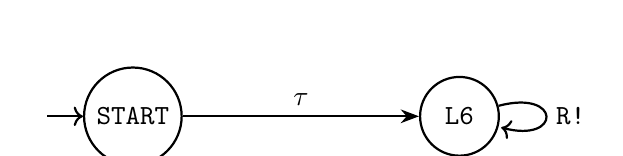
\begin{tikzpicture}[
    node distance=3cm,
    every state/.style={thick, minimum size=1cm},
    every edge/.style={draw, -Stealth, thick},
]
  \node[state, initial, initial text=] (s0) {\texttt{START}};
  \node[state, right=of s0] (s1) {\texttt{L6}};
  \path (s0) edge node[above] {$\tau$} (s1);
  \path (s1) edge[loop right] node[right] {\texttt{R!}} (s1);
\end{tikzpicture}
\end{center}

After initialization ($\tau$), the producer enters a single-state
cycle, sending on~\texttt{R} forever.

%----------------------------------------------------------------------
\subsection{Consumer LTS}
%----------------------------------------------------------------------

Applying the same algorithm to the consumer:

\begin{center}
\begin{tabular}{llll}
\toprule
\textbf{Block} & \textbf{Action} & \textbf{Target} & \textbf{Reason} \\
\midrule
\texttt{START} & $\tau$           & \texttt{L16}    & No blocking stmt \\
\texttt{L16}   & \texttt{L?}      & \texttt{L16}    & First blocking stmt is \texttt{recv L} \\
\bottomrule
\end{tabular}
\end{center}

The resulting LTS for the Consumer:

\begin{align*}
S   &= \{\texttt{START},\; \texttt{L16}\} \\
s_0 &= \texttt{START} \\
A   &= \{\texttt{L?}\} \\
{\to} &= \{(\texttt{START}, \tau, \texttt{L16}),\;
           (\texttt{L16}, \texttt{L?}, \texttt{L16})\}
\end{align*}

\begin{center}
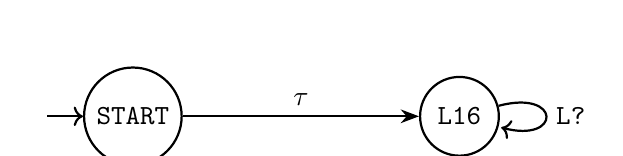
\begin{tikzpicture}[
    node distance=3cm,
    every state/.style={thick, minimum size=1cm},
    every edge/.style={draw, -Stealth, thick},
]
  \node[state, initial, initial text=] (s0) {\texttt{START}};
  \node[state, right=of s0] (s1) {\texttt{L16}};
  \path (s0) edge node[above] {$\tau$} (s1);
  \path (s1) edge[loop right] node[right] {\texttt{L?}} (s1);
\end{tikzpicture}
\end{center}

The consumer has the same structure: initialization followed by an
infinite receive loop.

%======================================================================
\section{The Aldebaran \texttt{.aut} Format}
%======================================================================

The Aldebaran \texttt{.aut} format is a simple textual representation
of labelled transition systems, originally developed for the CADP
toolbox~\cite{cadp}.  It consists of a header line followed by one
line per transition:

\begin{Verbatim}[samepage=true,xleftmargin=2em]
des (initial_state, num_transitions, num_states)
(source, "action", target)
...
\end{Verbatim}

States are represented as integers starting from~0, with the initial
state always at index~0.  Action labels are quoted strings.

%----------------------------------------------------------------------
\subsection{Producer \texttt{.aut} Output}
%----------------------------------------------------------------------

\begin{Verbatim}[samepage=true,xleftmargin=2em]
des (0, 2, 2)
(0, "tau", 1)
(1, "R!", 1)
\end{Verbatim}

State~0 is \texttt{START}, state~1 is \texttt{L6}.

%----------------------------------------------------------------------
\subsection{Consumer \texttt{.aut} Output}
%----------------------------------------------------------------------

\begin{Verbatim}[samepage=true,xleftmargin=2em]
des (0, 2, 2)
(0, "tau", 1)
(1, "L?", 1)
\end{Verbatim}

State~0 is \texttt{START}, state~1 is \texttt{L16}.

The \texttt{.aut} format is interoperable with external verification
tools such as CADP and mCRL2, which can analyze or compose the
per-process LTSs.

%======================================================================
\section{Using the Tools}
%======================================================================

The LTS extraction is available through the Scheme interface of
\texttt{cspc}.  The following examples assume the environment variable
\texttt{M3UTILS} points to the m3utils root directory.

%----------------------------------------------------------------------
\subsection{Extracting a Single Process LTS}
%----------------------------------------------------------------------

To compile a single \texttt{.scm} parse tree and extract its LTS:

\begin{lstlisting}
(load (string-append (Env.Get "M3UTILS") "/csp/src/setup.scm"))
(define lts (extract-process-lts! "ProdCons_46_Producer.scm"))
\end{lstlisting}

The function \texttt{extract-process-lts!}\ loads the parse tree,
runs the 9-pass compiler, and returns an LTS object.  It also
pretty-prints the LTS to standard output.

%----------------------------------------------------------------------
\subsection{Extracting All Processes in a System}
%----------------------------------------------------------------------

To extract LTSs for every process type in a \texttt{.sys} file:

\begin{lstlisting}
(load (string-append (Env.Get "M3UTILS") "/csp/src/setup.scm"))
(load (string-append (Env.Get "M3UTILS") "/csp/src/cspbuild.scm"))
(define results (extract-system-lts! "build_prodcons.sys"))
\end{lstlisting}

This returns an association list mapping process names to LTS objects:
\begin{lstlisting}
(("ProdCons.Producer" . <lts>) ("ProdCons.Consumer" . <lts>))
\end{lstlisting}

The \texttt{.sys} file and referenced \texttt{.csp} files must be in
the current directory (or accessible by \texttt{cspfe}).

%----------------------------------------------------------------------
\subsection{Writing \texttt{.aut} Files}
%----------------------------------------------------------------------

To export an LTS in Aldebaran format:

\begin{lstlisting}
(write-lts-aut lts "producer.aut")
\end{lstlisting}

%----------------------------------------------------------------------
\subsection{Inspecting the LTS Programmatically}
%----------------------------------------------------------------------

The LTS object supports the following accessors:

\begin{center}
\begin{tabular}{ll}
\toprule
\textbf{Accessor} & \textbf{Returns} \\
\midrule
\texttt{(lts-states lts)}      & List of state symbols \\
\texttt{(lts-initial lts)}     & Initial state symbol \\
\texttt{(lts-alphabet lts)}    & List of non-$\tau$ actions \\
\texttt{(lts-transitions lts)} & List of \texttt{(src action dst)} triples \\
\bottomrule
\end{tabular}
\end{center}

Actions are represented as \texttt{(send~$P$)} or
\texttt{(recv~$P$)} for channel operations, and the symbol
\texttt{tau} for internal transitions.

%======================================================================
\section{What the LTS Tells Us}
%======================================================================

Even these simple two-state LTSs reveal useful information about the
processes:

\begin{description}
\item[Determinism.]
  Both processes are deterministic: from every reachable state,
  there is exactly one enabled action.  The producer always sends;
  the consumer always receives.

\item[No deadlock (per-process).]
  Neither process can reach a state with no outgoing transitions.
  Both cycle forever through their communication loops.

\item[No livelock (per-process).]
  A livelock would require a cycle consisting entirely of $\tau$
  transitions---an infinite loop of internal computation with no
  visible progress.  Both LTSs have exactly one $\tau$ transition
  (the initialization step), which leads to a state with a visible
  channel action.  There are no $\tau$-only cycles.

\item[Single-channel interface.]
  The producer's alphabet is $\{\texttt{R!}\}$ and the consumer's is
  $\{\texttt{L?}\}$.  After port binding through the system file,
  these map to complementary operations on the same channel~\texttt{c}.
\end{description}

%======================================================================
\section{Looking Ahead: Product Composition}
%======================================================================

Phase~1 extracts the LTS of each process in isolation.  Phase~2 will
compose these per-process LTSs into a \emph{product LTS} representing
the entire system.

The composition follows the standard CSP parallel composition rule:
processes synchronize on shared channel events and interleave on
independent actions.  For the producer-consumer system, the
synchronization alphabet is $\{\texttt{c!},\, \texttt{c?}\}$---the
producer's \texttt{R!}\ and the consumer's \texttt{L?}\ both refer to
channel~\texttt{c} and must occur together.

The product state space is small:

\begin{center}
\begin{tabular}{cll}
\toprule
\textbf{Product State} & \textbf{Producer} & \textbf{Consumer} \\
\midrule
$(s_0, s_0)$  & \texttt{START} & \texttt{START} \\
$(s_0, s_1)$  & \texttt{START} & \texttt{L16} \\
$(s_1, s_0)$  & \texttt{L6}    & \texttt{START} \\
$(s_1, s_1)$  & \texttt{L6}    & \texttt{L16} \\
\bottomrule
\end{tabular}
\end{center}

From the product state $(\texttt{L6}, \texttt{L16})$, the producer
wants to send and the consumer wants to receive---they synchronize
successfully, and the system loops back to $(\texttt{L6},
\texttt{L16})$.  No product state is a deadlock (a state where no
component can make progress).  This system is deadlock-free.

For more complex systems with multiple channels, guarded selections,
and data-dependent branching, the product state space grows
combinatorially.  Phase~3 of the verification roadmap addresses this
with partial-order reduction, symmetry reduction, and data
abstraction.

%======================================================================
\section{References}
%======================================================================

\begin{thebibliography}{99}

\bibitem{feasibility}
M.~Nystr\"om,
``Formal Verification for the Fulcrum CSP Toolchain: Feasibility Study
and Project Plan,''
Technical report, 2025.

\bibitem{hoare1985}
C.~A.~R. Hoare,
\emph{Communicating Sequential Processes},
Prentice Hall, 1985.
Available online: \url{http://www.usingcsp.com/}

\bibitem{cadp}
H.~Garavel, F.~Lang, R.~Mateescu, W.~Serwe,
``CADP 2011: A Toolbox for the Construction and Analysis of
Distributed Processes,''
\emph{International Journal on Software Tools for Technology Transfer},
vol.~15, no.~2, pp.~89--107, 2013.

\end{thebibliography}

\end{document}
